\section{Abstract Argumentation Framework, AAF}
%Système d'argumentation abstrait}
\label{sec:AAF}

This section briefly recalls the basics of~\cite{dung_acceptability_1995}'s AAF.

\begin{definition}\label{def:AAF}
    An \emph{abstract argumentation framework}~$AAF$ is a couple~${AF = (A,R)}$, where~$A$ is a finite set of arguments and~$R$ is a set of \emph{attacks} corresponding to a binary relation~$A \times A$. An argument~$x\in A$ attacks~$y\in A$ if~$(x,y)\in R$.
\end{definition}

As $R$ is a binary relation with a finite support, an AAF can be represented using a graph.

\begin{example}
\label{ex:IRM_ou_radio}

To illustrate these notions, we introduce an argumentative scenario modelling the interaction between a requesting physician, D, and a radiologist, R, concerning an examination of a $n$ month old baby for pathology Z.
\\ \textit{D:} Can you do an X-ray scanner (CT) for this baby? ($a$) \\
\textit{R:} It is better for a baby to avoid ionising radiations. ($b$) \\
\textit{R:} I can suggest an MRI (magnetic resonance imaging) in two days' time. ($c$) \\
\textit{D:} Can Z be seen on an MRI? ($d$) \\
\textit{R:} Yes, of course! If you want confirmation, look at the guide to good radiology practice. ($e$) \\
\textit{D:} But a baby might move and so you might not be able to get the information you are looking for because the image may be artefacted. ($f$) \\
\textit{R:} Do not worry, I am used to doing MRI for babies. ($g$) \\
\textit{D:} Does not it cost the hospital a lot more to do an MRI?~($h$) I also have to check with the patient's family because it might cost them more. ($i$) \\
\textit{R:}  No problem here. The high cost includes the experience gained by my team so that in the future this kind of delicate examination can be performed without me. ($j$) \\
\textit{D:} I have just spoken to the family, no problem with the MRI, the exam is refunded.~($k$) \\
\textit{D:} 
However, the family is not comfortable with the idea of having to wait two days, could not you do the exam before?~($l$)\\
\textit{R:} No my schedule for today is already full. My next slot is in two days, as I told you.~($m$)

After this discussion, the decision is made to schedule an MRI in two days' time. But later that day, the doctor receives a call from the family saying that the baby is really not well and insisting on the urgency of the examination. Therefore, the doctor contacts the radiologist to add a final argument.\\
\textit{D:} It is very urgent for the baby, we need a place today! ($n$)

From this dialogue, we can extract manually arguments and their relations to create the AAF represented in Figure~\ref{fig:ex_radio} with the following arguments:~$\{ \textbf{a}$: Scanner, $b$: Ionising radiation, $\textbf{c}$: MRI in two days, $d$: Z not visible by MRI, $e$: Z visible by MRI, $f$: Difficult conditions, $g$: High experience, $h$: High cost for the hospital, $i$: High cost for the patient, $j$: Not problematic for the hospital, $k$: The family is covered for an MRI, $\textbf{l}$: MRI today, $m$: No availability today, $n$: It is an emergency!$\}$. Arguments $a,c,l$ are called the decision variables, their acceptance being the criterion triggering a decision: CT, MRI in two days, or MRI today.

The obtained argumentation system is a possibility of graph that can be extracted from this dialogue.
%, a proposition that we will use later. It is possible to do 
The extraction process can be done automatically
%in an automated manner through a set of methods called 
using so-called argument mining methods~\cite{lippi2016argumentation}.

\begin{figure}[t]
    \centering
    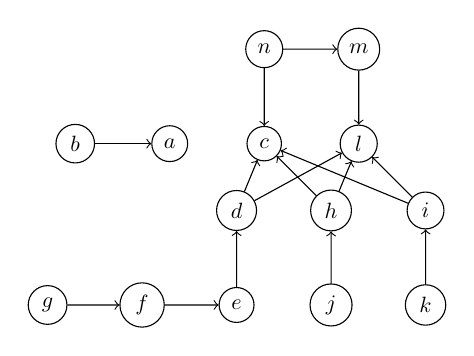
\begin{tikzpicture}[scale=0.8,transform shape, node distance={15mm}, main/.style = {draw, circle}]
            
                \node[main] (1) {$a$}; 
                \node[main] (2) [left of=1] {$b$};
                \node[main] (3) [right of=1] {$c$};
                \node[main] (4) [right of=3] {$l$};
                \node[main] (5) [below right of=3] {$h$};
                \node[main] (6) [left of=5] {$d$};
                \node[main] (7) [right of=5] {$i$};
                \node[main] (8) [above of=3] {$n$};
                \node[main] (9) [above of=4] {$m$};
                \node[main] (10) [below of=6] {$e$};
                \node[main] (11) [below of=5] {$j$};
                \node[main] (12) [below of=7] {$k$};
                \node[main] (13) [left of=10] {$f$};
                \node[main] (14) [left of=13] {$g$};
                
                
                
                \draw[->] (2) -- (1);
                \draw[->] (5) -- (3);
                \draw[->] (6) -- (3);
                \draw[->] (7) -- (3);
                \draw[->] (8) -- (3);
                \draw[->] (5) -- (4);
                \draw[->] (6) -- (4);
                \draw[->] (7) -- (4);
                \draw[->] (9) -- (4);
                \draw[->] (10) -- (6);
                \draw[->] (13) -- (10);
                \draw[->] (14) -- (13);
                \draw[->] (11) -- (5);
                \draw[->] (12) -- (7);
                \draw[->] (8) -- (9);
                
            \end{tikzpicture}
    \caption{
    %Graphe d'argumentation associé à l'exemple
    Argumentation graph associated with Example~\ref{ex:IRM_ou_radio}.}
    \label{fig:ex_radio}
\end{figure}
\end{example}

%\textbf{Remark --} 
Note that this is a static representation of the dialogue from which any notion of temporality has been erased. Thus, if the arguments had been stated in a different order, it would not change the graph. This will be important to address causality in Section~\ref{sec:discu_causalite}.

%\medskip
%\label{sec:def_AAF}

Once an argumentation graph has been constructed, it is possible to reason on it to determine sets of arguments that can be considered as accepted.

The \emph{set of direct attackers} of~$x \in A$ is denoted by~$Att_{x}=\{ y\in A \mid (y,x)\in R\}$. A set~$S$ is \emph{conflict-free} if~${\forall (x,y) \in S^2}$, $(x,y)\notin R$. An argument~$x \in A$ is \emph{acceptable} by~$S$ if~$\forall y\in %Att_a, 
Att_x, \exists z \in S \cap Att_y$.

Then an \emph{admissible set}~$S$ is defined as a conflict-free set whose 
elements are all acceptable by~$S$ itself. 
%in which all these elements are acceptable by the set. 
For an acyclic graph, this is the only extension-based semantics as all others coincide
%in a single, admissible extension, and will therefore not be
with it and are therefore not discussed here~\cite{rahwan2009argumentation}. 
% In addition to these definitions, we can also define extension-based semantics~\cite{rahwan2009argumentation}. These are properties that must be satisfied by a set of arguments in order for it to be accepted. In the case of acyclic graphs, all these semantics coincide in a single, admissible extension, and will therefore not be discussed here~\cite{rahwan2009argumentation}.

\addtocounter{example}{-1}
\begin{example} (continued) --
The argument graph
%obtained to model the dialogue between the radiologist and the doctor 
is acyclic. To determine the set of acceptable arguments, it is sufficient to start from the non-attacked arguments, here~${b,g,j,k,n}$. They are accepted by default. Then, an argument attacked by at least one accepted argument cannot be accepted. By applying this rule, we obtain that argument $l$ is accepted, in contrast to $a$ and $c$. Therefore, the final decision is to perform an emergency MRI today.
\end{example}
